% Options for packages loaded elsewhere
\PassOptionsToPackage{unicode}{hyperref}
\PassOptionsToPackage{hyphens}{url}
%
\documentclass[
  man,floatsintext]{apa6}
\usepackage{amsmath,amssymb}
\usepackage{iftex}
\ifPDFTeX
  \usepackage[T1]{fontenc}
  \usepackage[utf8]{inputenc}
  \usepackage{textcomp} % provide euro and other symbols
\else % if luatex or xetex
  \usepackage{unicode-math} % this also loads fontspec
  \defaultfontfeatures{Scale=MatchLowercase}
  \defaultfontfeatures[\rmfamily]{Ligatures=TeX,Scale=1}
\fi
\usepackage{lmodern}
\ifPDFTeX\else
  % xetex/luatex font selection
\fi
% Use upquote if available, for straight quotes in verbatim environments
\IfFileExists{upquote.sty}{\usepackage{upquote}}{}
\IfFileExists{microtype.sty}{% use microtype if available
  \usepackage[]{microtype}
  \UseMicrotypeSet[protrusion]{basicmath} % disable protrusion for tt fonts
}{}
\makeatletter
\@ifundefined{KOMAClassName}{% if non-KOMA class
  \IfFileExists{parskip.sty}{%
    \usepackage{parskip}
  }{% else
    \setlength{\parindent}{0pt}
    \setlength{\parskip}{6pt plus 2pt minus 1pt}}
}{% if KOMA class
  \KOMAoptions{parskip=half}}
\makeatother
\usepackage{xcolor}
\usepackage{graphicx}
\makeatletter
\def\maxwidth{\ifdim\Gin@nat@width>\linewidth\linewidth\else\Gin@nat@width\fi}
\def\maxheight{\ifdim\Gin@nat@height>\textheight\textheight\else\Gin@nat@height\fi}
\makeatother
% Scale images if necessary, so that they will not overflow the page
% margins by default, and it is still possible to overwrite the defaults
% using explicit options in \includegraphics[width, height, ...]{}
\setkeys{Gin}{width=\maxwidth,height=\maxheight,keepaspectratio}
% Set default figure placement to htbp
\makeatletter
\def\fps@figure{htbp}
\makeatother
\setlength{\emergencystretch}{3em} % prevent overfull lines
\providecommand{\tightlist}{%
  \setlength{\itemsep}{0pt}\setlength{\parskip}{0pt}}
\setcounter{secnumdepth}{-\maxdimen} % remove section numbering
% Make \paragraph and \subparagraph free-standing
\ifx\paragraph\undefined\else
  \let\oldparagraph\paragraph
  \renewcommand{\paragraph}[1]{\oldparagraph{#1}\mbox{}}
\fi
\ifx\subparagraph\undefined\else
  \let\oldsubparagraph\subparagraph
  \renewcommand{\subparagraph}[1]{\oldsubparagraph{#1}\mbox{}}
\fi
\newlength{\cslhangindent}
\setlength{\cslhangindent}{1.5em}
\newlength{\csllabelwidth}
\setlength{\csllabelwidth}{3em}
\newlength{\cslentryspacingunit} % times entry-spacing
\setlength{\cslentryspacingunit}{\parskip}
\newenvironment{CSLReferences}[2] % #1 hanging-ident, #2 entry spacing
 {% don't indent paragraphs
  \setlength{\parindent}{0pt}
  % turn on hanging indent if param 1 is 1
  \ifodd #1
  \let\oldpar\par
  \def\par{\hangindent=\cslhangindent\oldpar}
  \fi
  % set entry spacing
  \setlength{\parskip}{#2\cslentryspacingunit}
 }%
 {}
\usepackage{calc}
\newcommand{\CSLBlock}[1]{#1\hfill\break}
\newcommand{\CSLLeftMargin}[1]{\parbox[t]{\csllabelwidth}{#1}}
\newcommand{\CSLRightInline}[1]{\parbox[t]{\linewidth - \csllabelwidth}{#1}\break}
\newcommand{\CSLIndent}[1]{\hspace{\cslhangindent}#1}
\ifLuaTeX
\usepackage[bidi=basic]{babel}
\else
\usepackage[bidi=default]{babel}
\fi
\babelprovide[main,import]{english}
% get rid of language-specific shorthands (see #6817):
\let\LanguageShortHands\languageshorthands
\def\languageshorthands#1{}
% Manuscript styling
\usepackage{upgreek}
\captionsetup{font=singlespacing,justification=justified}

% Table formatting
\usepackage{longtable}
\usepackage{lscape}
% \usepackage[counterclockwise]{rotating}   % Landscape page setup for large tables
\usepackage{multirow}		% Table styling
\usepackage{tabularx}		% Control Column width
\usepackage[flushleft]{threeparttable}	% Allows for three part tables with a specified notes section
\usepackage{threeparttablex}            % Lets threeparttable work with longtable

% Create new environments so endfloat can handle them
% \newenvironment{ltable}
%   {\begin{landscape}\centering\begin{threeparttable}}
%   {\end{threeparttable}\end{landscape}}
\newenvironment{lltable}{\begin{landscape}\centering\begin{ThreePartTable}}{\end{ThreePartTable}\end{landscape}}

% Enables adjusting longtable caption width to table width
% Solution found at http://golatex.de/longtable-mit-caption-so-breit-wie-die-tabelle-t15767.html
\makeatletter
\newcommand\LastLTentrywidth{1em}
\newlength\longtablewidth
\setlength{\longtablewidth}{1in}
\newcommand{\getlongtablewidth}{\begingroup \ifcsname LT@\roman{LT@tables}\endcsname \global\longtablewidth=0pt \renewcommand{\LT@entry}[2]{\global\advance\longtablewidth by ##2\relax\gdef\LastLTentrywidth{##2}}\@nameuse{LT@\roman{LT@tables}} \fi \endgroup}

% \setlength{\parindent}{0.5in}
% \setlength{\parskip}{0pt plus 0pt minus 0pt}

% Overwrite redefinition of paragraph and subparagraph by the default LaTeX template
% See https://github.com/crsh/papaja/issues/292
\makeatletter
\renewcommand{\paragraph}{\@startsection{paragraph}{4}{\parindent}%
  {0\baselineskip \@plus 0.2ex \@minus 0.2ex}%
  {-1em}%
  {\normalfont\normalsize\bfseries\itshape\typesectitle}}

\renewcommand{\subparagraph}[1]{\@startsection{subparagraph}{5}{1em}%
  {0\baselineskip \@plus 0.2ex \@minus 0.2ex}%
  {-\z@\relax}%
  {\normalfont\normalsize\itshape\hspace{\parindent}{#1}\textit{\addperi}}{\relax}}
\makeatother

\makeatletter
\usepackage{etoolbox}
\patchcmd{\maketitle}
  {\section{\normalfont\normalsize\abstractname}}
  {\section*{\normalfont\normalsize\abstractname}}
  {}{\typeout{Failed to patch abstract.}}
\patchcmd{\maketitle}
  {\section{\protect\normalfont{\@title}}}
  {\section*{\protect\normalfont{\@title}}}
  {}{\typeout{Failed to patch title.}}
\makeatother

\usepackage{xpatch}
\makeatletter
\xapptocmd\appendix
  {\xapptocmd\section
    {\addcontentsline{toc}{section}{\appendixname\ifoneappendix\else~\theappendix\fi\\: #1}}
    {}{\InnerPatchFailed}%
  }
{}{\PatchFailed}
\keywords{big team, science, authorship, credit}
\usepackage{lineno}

\linenumbers
\usepackage{csquotes}
\ifLuaTeX
  \usepackage{selnolig}  % disable illegal ligatures
\fi
\IfFileExists{bookmark.sty}{\usepackage{bookmark}}{\usepackage{hyperref}}
\IfFileExists{xurl.sty}{\usepackage{xurl}}{} % add URL line breaks if available
\urlstyle{same}
\hypersetup{
  pdftitle={Who does big team science?},
  pdfauthor={Erin M. Buchanan1 \& Savannah C. Lewis2},
  pdflang={en-EN},
  pdfkeywords={big team, science, authorship, credit},
  hidelinks,
  pdfcreator={LaTeX via pandoc}}

\title{Who does big team science?}
\author{Erin M. Buchanan\textsuperscript{1} \& Savannah C. Lewis\textsuperscript{2}}
\date{}


\shorttitle{Big Team Science}

\authornote{

Erin M. Buchanan is a Professor of Cognitive Analytics at Harrisburg University of Science and Technology. Savannah C. Lewis is a graduate student at the University of Alabama.

Thank you to Dwayne Lieck for providing an extensive list of large scale projects for this manuscript.

The authors made the following contributions. Erin M. Buchanan: Conceptualization, Data curation, Formal Analysis, Methodology, Project administration, Visualization, Writing -- original draft, Writing -- review \& editing; Savannah C. Lewis: Conceptualization, Data curation, Methodology, Project administration, Writing -- original draft, Writing -- review \& editing.

Correspondence concerning this article should be addressed to Erin M. Buchanan, 326 Market St., Harrisburg, PA 17101. E-mail: \href{mailto:ebuchanan@harrisburgu.edu}{\nolinkurl{ebuchanan@harrisburgu.edu}}

}

\affiliation{\vspace{0.5cm}\textsuperscript{1} Harrisburg University of Science and Technology\\\textsuperscript{2} University of Alabama}

\abstract{%
This paper examined the nature of publications in Big Team Science (BTS) - large-scale collaborations between multiple researchers at multiple institutions. As interest in BTS increases, it is useful to explore who is currently involved in BTS projects to determine diversity in both research subject and researcher representation. The types of publication outlets, number of publications, and subject areas of publication are presented to summarize the publications in BTS. Information about authors included in BTS will be presented including career length, numbers of publications/impact variables, education, and affiliation. Last, we will explore the representation of geopolitical regions by examining affiliation location to explore the impact of BTS on the de-WEIRD movement to diversify researcher representation. REWRITE THIS
}



\begin{document}
\maketitle

According to the Oxford English dictionary, collaboration is two or more
people working together to achieve a certain goal (OED, 2016).
Collaboration in scientific endeavors involves multiple researchers at
(potentially) multiple institutions to communicate and work together to
advance knowledge in their chosen field. Collaboration can manifest
uniquely in each project dependent on the skill sets, hypotheses, and
perspectives of collaborators. While collaboration is not new in
science, the current interest of ``big team science'' is increasing
(Coles, Hamlin, Sullivan, Parker, \& Altschul, 2022; Forscher et al., 2020; N. Stewart, Chandler, \& Paolacci, 2017). Big team science projects
and/or organizations utilize and run on large-scale collaboration to
ensure that diverse populations and ideas are brought into research
projects, which in turn allows for more reliability and generalizability
in the results and method of the study. For this study, Big Team Science
(BTS) will be defined as a collaboration of ten or more authors from at
least ten different institutions.

BTS appears to be increasing as a result of two sources: 1) increasing
globalization and technology that allows for real-time interdisciplinary
research, and 2) increasing interest in reproducibility, replication,
and generalizability (Maxwell, Lau, \& Howard, 2015; Nelson, Simmons, \& Simonsohn, 2018; Zwaan, Etz, Lucas, \& Donnellan, 2018).
Technological advances have provided easier ways to collaborate with
people who are from other universities and countries through document
sharing platforms (e.g., Google, GitHub, and the Open Science
Framework), video chatting platforms (e.g., Zoom, Microsoft Teams), and
messaging and project management platforms (e.g., Slack, Trello,
when2meet, etc.). The credibility movement seems to suggest that by
having both collaborations that span across the globe and subfields of
research areas, age groups, and education levels should help to drive science in the path of better materials, reliability,
generalizability and more robust sample sizes (when necessary) in a study
(Auspurg \& Brüderl, 2021; LeBel, McCarthy, Earp, Elson, \& Vanpaemel, 2018; Brian A. Nosek \& Lakens, 2014a).

The credibility movement was originally defined by a focus on large
scale replications using in collaborative environments (Vazire, Schiavone, \& Bottesini, 2022).
Generally, the movement appears to have been driven by early career researchers
(i.e., those who are within five years of their first appointment)
(Maizey \& Tzavella, 2019); however, there are no large meta-scientific
investigations on this specific topic to date. Potentially, the lack of
investigation is tied to the newness of the large-scale research in many
fields, as it is only in recent years that publications like the Open
Science Collaboration (Open Science Collaboration, 2015), Many Labs
Collaborations (Buttrick et al., 2020; Ebersole et al., 2016, 2020; Richard A. Klein et al., 2022; for example, Richard A. Klein et al., 2018; Mathur et al., 2020; Skorb et al., 2020) or the first papers
from the Psychological Science Accelerator (Bago et al., 2022; Dorison et al., 2022; Jones et al., 2021; Legate et al., 2022; Moshontz et al., 2018; Wang et al., 2021). Generally, the
researcher incentive for replication was low: journals often prioritize
``novel'' or new results which led to rejection of replication manuscripts
and publication bias (Franco, Malhotra, \& Simonovits, 2014; Hubbard \& Armstrong, 1997; Brian A. Nosek, Spies, \& Motyl, 2012), the
``failure'' to replicate was often placed on the replication team as ``bad
science'' rather than a careful consideration of publication biases and
(potential) questionable research practices (Ioannidis, 2015; Richard A. Klein et al., 2022; Maxwell et al., 2015), and why should someone want to spend time and
resources on an answer we already ``know'' (Isager et al., 2021a, 2021b)?

However, the success and interest in the large-scale reproducibility
projects (Errington et al., 2021; Open Science Collaboration, 2015), paired
with the meta-scientific publications focusing on researcher practices
and incentive structures (John, Loewenstein, \& Prelec, 2012; Silberzahn et al., 2018) led to a
change in journal guidelines and incentives for researchers interested
in participating in large-scale replication studies (Grahe, 2014; Kidwell et al., 2016; Mayo-Wilson et al., 2021; B. A. Nosek et al., 2015). For example, the support
for Registered Reports, papers accepted before the data has been
collected (Brian A. Nosek \& Lakens, 2014b; S. Stewart et al., 2020), and entire sub-sections of
journals devoted to only replication studies (e.g., \emph{Nature, Royal Society Open Science, Advances in Methods and Practices in Psychological Science}) has allowed researchers to invest in projects that they know
should be published when the project is complete. Further, the
implementation of the Transparency and Openness Guidelines (B. A. Nosek et al., 2015)
and the Contributor Role Taxonomy (CRediT) system (Allen, O'Connell, \& Kiermer, 2019) have
pushed journals and researchers to promote more open, inclusive
publication practices.

The credibility movement has been mirrored by the calls for
diversification or de-WEIRDing (e.g., Western, Educated, Industrialized,
Rich, and Democratic) scientific research (Henrich, Heine, \& Norenzayan, 2010; Newson, Buhrmester, Xygalatas, \& Whitehouse, 2021; Rad, Martingano, \& Ginges, 2018) by improving representation in research samples. Like the
large-scale studies in Physics ({``A Philosophical Case for Big Physics,''} 2021; Castelnovo, Florio, Forte, Rossi, \& Sirtori, 2018) and
Biology (Collins, Morgan, \& Patrinos, 2003), the social sciences struggle to represent the
breadth of humanity across both researcher and population
characteristics. Now, grassroots organizations, such as the
Psychological Science Accelerator (Moshontz et al., 2018), ManyBabies
(\url{https://manybabies.github.io/}), NutNet (\url{https://nutnet.org/}), and
DRAGNet (\url{https://dragnetglobal.weebly.com/}) can begin to tackle these
issues by recruiting research labs from all over the globe to provide
diversity in geographic, linguistic, and researcher representation.
Publications have examined the global understanding of morality, face
processing, COVID-19 information signaling, and more (Bago et al., 2022; Dorison et al., 2022; Jones et al., 2021; Legate et al., 2022; Van Bavel et al., 2022; Wang et al., 2021). While
these organizations and one-time groups for BTS studies have provided an
incredible wealth of data for the scientific community, we do not yet
know exactly \emph{who} is involved with, and benefits from, the BTS and
credibility movement. Publications on BTS generally explore challenges,
lessons learned, and the need for BTS (Coles et al., 2022; Forscher et al., 2020).

Therefore, the goal of this manuscript is to examine the \emph{people}
involved in BTS projects. We specifically examined the themes of inclusivity, research careers, and research globalization. We see an
increasing interest and number of publications in BTS but we do not yet know if
this uptick in large-scale projects has diversified the \emph{people}
involved in BTS. While a few publications have noted that BTS appears to
be early career researchers (Maizey \& Tzavella, 2019), no one has systematically
investigated this perception. Further, it is unclear if the focus of
de-WEIRDing science has only focused on the representation of the
research participants or if it has also improved the representation of
researchers outside of North America and Europe. Last, who runs these
BTS projects? Do we see an increase in diversity for the authors who
generally receive the most credit for these projects (i.e., first
several author(s) and last author)? As hiring and promoting practices
often place a heavy weight on publications and especially ``influential''
publications, it becomes necessary to critically examine the
representation present in authorship in BTS projects.

\hypertarget{research-questions}{%
\section{Research Questions}\label{research-questions}}

\begin{itemize}
\tightlist
\item
  Research Question 1: What publication sources publish big team
  science papers?
\item
  Research Question 2: What are the types of articles that are being
  published in big team science?
\item
  Research Question 3: Who is involved in big team science?
\end{itemize}

This manuscript was preregistered with the same conceptual ideas using Google Scholar and ORC-ID databases (\url{https://osf.io/f2dtr}) but then was updated with access to the Scopus database for a broader picture of BTS projects (\url{https://osf.io/fheun}). All materials and code can be found on our OSF page: \url{https://osf.io/cgx6u/} or corresponding GitHub archive: \url{https://github.com/doomlab/big_team_who}.

\hypertarget{method}{%
\section{Method}\label{method}}

\hypertarget{publications}{%
\subsection{Publications}\label{publications}}

We have defined BTS publications as publications with at least ten
authors at ten different institutions that were published in
peer-reviewed journals or had posted a full paper pre-print. We used
data from 1970 and forward in the Scopus database, as it
is noted online that this time period includes cited references for
calculation of several of our variables described below. We will analyze
our results based on four subject areas present in the Scopus database: Physical Sciences,
Health Sciences, Social Sciences, and Life Sciences. We filtered the
database to include articles, articles in press, business articles,
conference papers, data papers, preprints, and surveys using Elsevier's
classification system. This project was supported by access to the Scopus database through the International Center for the Study of Research.

\hypertarget{data-curation}{%
\subsection{Data Curation}\label{data-curation}}

\hypertarget{rq1-publisher-information.}{%
\subsubsection{RQ1: Publisher Information.}\label{rq1-publisher-information.}}

We extracted the following information for publication sources: the name of the publication (source title), subject area (both the large four subject areas and the smaller four digit all science journal classification {[}ASJC{]} code), and the journal
impact using the Source Normalized Impact per Paper (SNIP).

\hypertarget{rq2-publication-information.}{%
\subsubsection{RQ2: Publication Information.}\label{rq2-publication-information.}}

For each publication of the identified BTS publications, we examined
the full four digit ASJC subject areas codes for each of the larger four
subject areas and the keywords present for these publications.

\hypertarget{rq3-author-information.}{%
\subsubsection{RQ3: Author Information.}\label{rq3-author-information.}}

The author list was extracted from each publication. Next, we used the author and affiliation arrays to curate a list of all publications and author information included in BTS papers to calculate the variables described below.

\textbf{\emph{Career Length}}. Career length for each author was defined as
the year of the first publication minus the current year listed for each author.

\textbf{\emph{Institution and Geopolitical Region}}. We used the affiliation
ids and country to gather information about the places of education
and/or employment for authors. Geopolitical region was created by binning these codes into United Nation Regions.

\textbf{\emph{Education}}. We collected degree information from the author table. Information on this variable is in the appendix.

\textbf{\emph{Types of Publications}}. We took information from the
publication type variable for each author's publications to present
information about the types of papers BTS authors publish. Information on this variable is in the appendix.

\textbf{\emph{Publication Metrics}}. For each author, we calculated the total
number of publications, and the h-index. The h-index represents the
highest \emph{h} number of publications that have at least \emph{h} citations. \emph{h}-count was only used for descriptive statistics.

\hypertarget{results}{%
\section{Results}\label{results}}

We used the 95\% confidence interval to make decisions on predictor or effect size differences from zero. The confidence interval that does not include zero would be considered different from zero (to four decimal places). We made no directional predictions.

\hypertarget{rq1-publisher-information.-1}{%
\subsection{RQ1: Publisher Information.}\label{rq1-publisher-information.-1}}

\emph{Number of articles}. The total number of articles included in this analysis was 510334 including 445301 Health Sciences articles, 228194
Physical Sciences articles, 26652 Social Sciences articles, and
307514 Life Sciences articles. Articles could be classified into
multiple categories. Figure \ref{fig:fig-pub-time} shows the number of articles published across time for each of the four large subject areas.

\begin{figure}
\centering
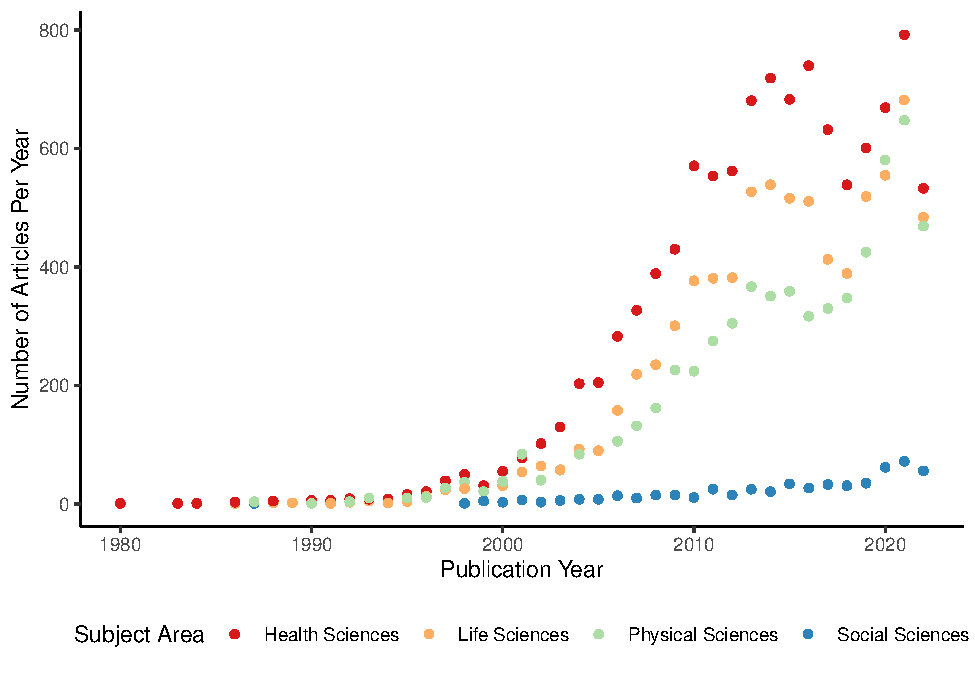
\includegraphics{manuscript_scopus_files/figure-latex/fig-pub-time-1.pdf}
\caption{\label{fig:fig-pub-time}Number of big-team science publications separated by four large subject areas across years.}
\end{figure}

\emph{Number of journals}. The number of distinct journals big team science articles were published
in was 14924 with 6559 journals in Health Sciences,
5787 journals in Physical Sciences, 2500
journals in Social Sciences, and 4187 journals in Life
Sciences. The descriptive statistics for the Source Normalized Impact
per Paper is presented the supplemental materials with a comparison for all papers.

\hypertarget{rq2-publication-information.-1}{%
\subsection{RQ2: Publication Information.}\label{rq2-publication-information.-1}}

Publication interest area was summarized by the four large subject areas creating a word cloud plot of the total number of publications within the ASJCs. Figure \ref{fig:fig-clouds} displays that the health sciences tends to publish within medicine and oncology, with a corresponding focus of cancer research and genetics for the life sciences. The physical sciences is mostly dominated by physics research, chemistry, and ecology. The BTS publications in the social sciences are mostly within psychology, education, and health.

\begin{figure}
\centering
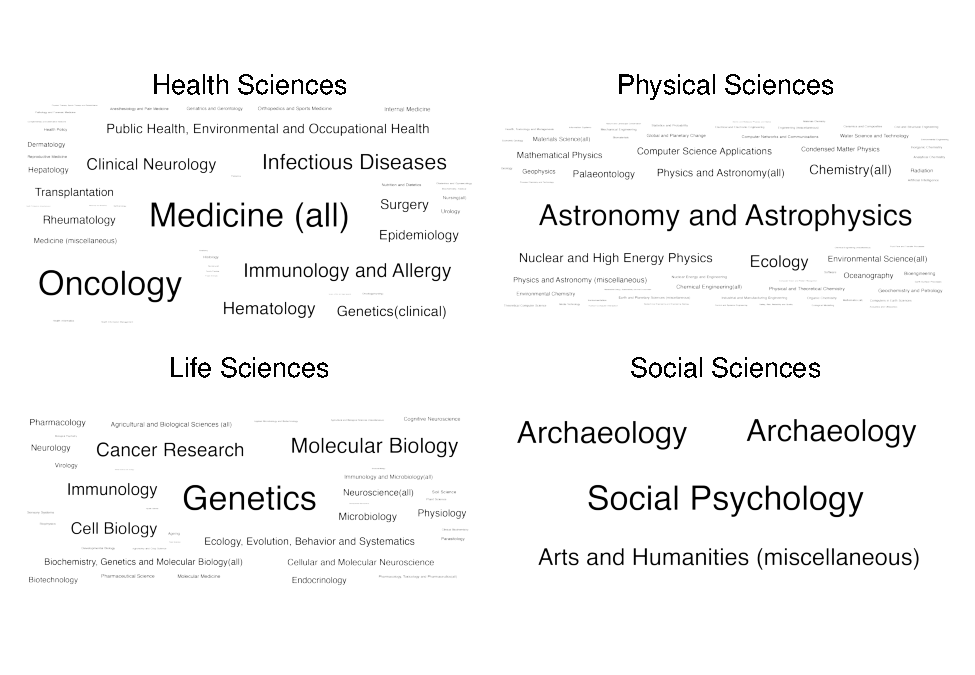
\includegraphics{manuscript_scopus_files/figure-latex/fig-clouds-1.pdf}
\caption{\label{fig:fig-clouds}Journal Areas for Big-Team Science Publications by Subject Area}
\end{figure}

\hypertarget{rq3-authors.}{%
\subsection{RQ3: Authors.}\label{rq3-authors.}}

The total number of unique authors across all publications was 510334. The mean number of authors per publication was \emph{M} = 49.31 (\emph{SD} = 212.98, \emph{Med} = 18) with a range of 10 to 5568. The median and average number of authors by subject area are displayed in Figure \ref{fig:fig-author-year}. In general, the average and median number of authors increased over time, with the exception of the skew in the physical sciences. Interestingly, the effect in the physical sciences appears to be declining toward the general trends seen in other areas in the last few decades.

\begin{figure}
\centering
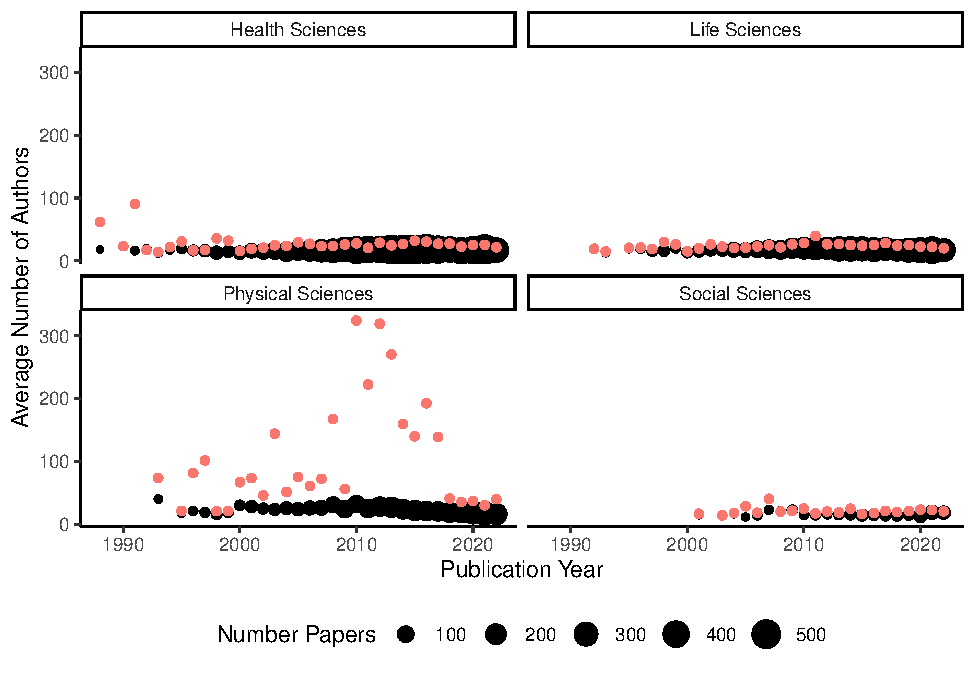
\includegraphics{manuscript_scopus_files/figure-latex/fig-author-year-1.pdf}
\caption{\label{fig:fig-author-year}Number of authors included on big-team science papers per year by subject area. Given the large skew in the data, the left panel presents the median number of authors per manuscript, and the right panel presents the average number of authors per manuscript by year.}
\end{figure}

\textbf{\emph{Career Length}}.

Figure \ref{fig:fig-career} portrays the average career length for authors involved in BTS publications across years. Career length was defined as the year of first publication minus the current year, and higher numbers mean longer careers. To analyze trends over time, we calculated the average career length for each publication (i.e., average author career lengths to create one score for each paper) and analyzed a regression analysis using career length to predict year of publication. In order to show variance between individuals, we calculated the standard deviation of career length for each publication and used variance as an additional predictor.

Negative career length slopes would indicate more young scholars in later years (i.e., lower average career length as time increases). Positive career length slopes would indicate older scholars in later years (i.e., higher average career length as time increases). Negative career variance slopes imply that variability decreases over the years, so the average career length is more homogeneous. Positive career length slopes imply that variability increases over the years, so the average career length is varied across individuals (i.e., different stages of scholars). Figure \ref{fig:fig-heatmap} displays the results for all regression analyses to compare coefficient strength across and within hypothesis.

All values for this analyses were different from zero. The slopes for the average career length were negative for all four subject areas, indicating a trend toward younger scientist involvement over time for each area, with the strongest effect in the Physical sciences. The coefficient for variability in career length was also negative for each of the four subject areas with the highest in the Physical sciences and lowest in the Life Sciences. This result indicates a decrease in the variability of career lengths over time, likely from two sources: 1) more publications with more authors, thus, lowering variance estimations, and 2) more young scholars overall. The effect sizes for this analysis were surprisingly large ranging from \(R^2\) to .25 to .47. All values and their confidence intervals can be found on our OSF page.

\begin{figure}
\centering
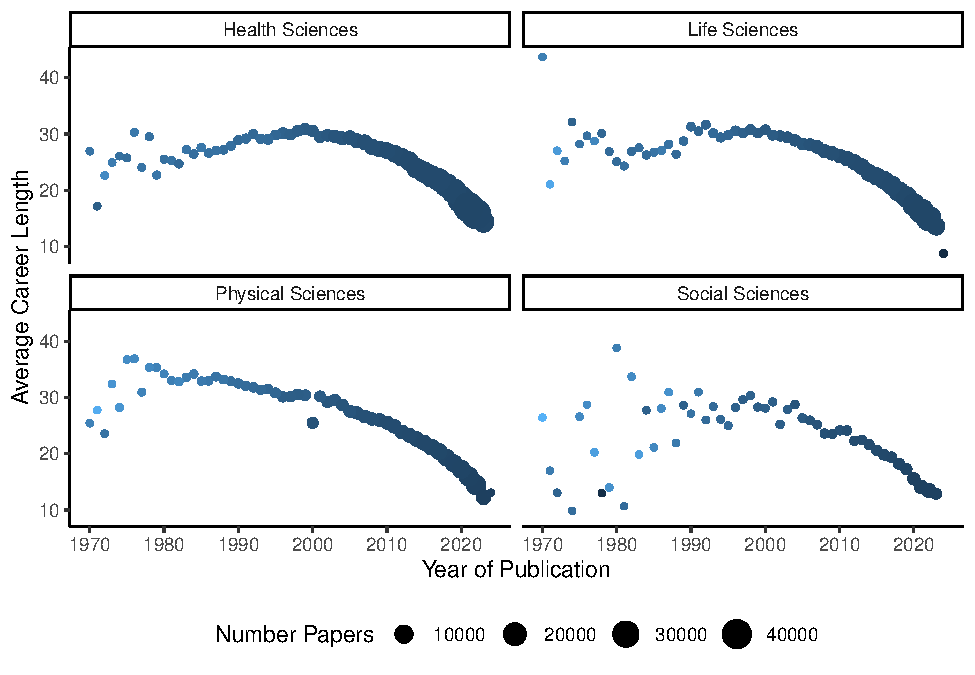
\includegraphics{manuscript_scopus_files/figure-latex/fig-career-1.pdf}
\caption{\label{fig:fig-career}Average career length for big-team science authors. Larger dots indicate more variability in career length for authors by averaging the standard deviation in career length for each manuscript within a year. The data has been filtered to at least 10 publications in a year for this graph.}
\end{figure}

\begin{verbatim}
## Warning in width_strings[fixed_areas[[i]]$cols] == "-1null" && length(w) == :
## 'length(x) = 3 > 1' in coercion to 'logical(1)'
\end{verbatim}

\begin{figure}
\centering
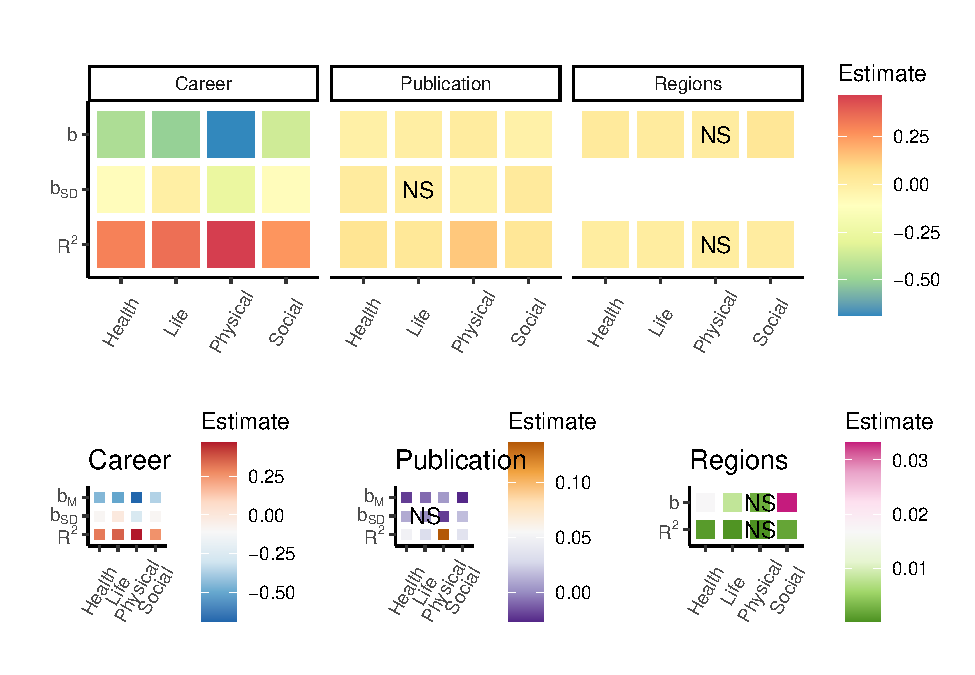
\includegraphics{manuscript_scopus_files/figure-latex/fig-heatmap-1.pdf}
\caption{\label{fig:fig-heatmap}Heatmap results of regression analyses for career length, number of publications, and geopolitical diversity in region. The top figure represents all results together for comparison across analyses. The bottom row represents individual heatmaps for each hypothesis to distinguish small differences between subject areas for those research questions. Non-significant results are indicated with NS on the plot.}
\end{figure}

\begin{verbatim}
## Warning in width_strings[fixed_areas[[i]]$cols] == "-1null" && length(w) == :
## 'length(x) = 3 > 1' in coercion to 'logical(1)'
\end{verbatim}

\textbf{\emph{Institution}}.

The total number of unique affiliation across all papers was 463876.

\textbf{\emph{Publication Metrics}}.

The average number of publications by authors on big team sciences
papers is \emph{M} = 38.37 (\emph{SD} =
102.54). The publication counts were averaged across
authors for each publication, and then these average publication counts
were averaged across publications \emph{M} = 162.50 (\emph{SD} =
155.17). The average variability (i.e., the average
standard deviation with authors of a manuscript) with publication counts
of a paper was \(M_{SD}\) = 164.27 (\(SD_{SD}\) =
127.21).

The same process was completed with \emph{h}-index for each author and
publication. The average \emph{h}-index for authors overall was \emph{M} =
33.65 (\emph{SD} = 127.34, \emph{Med} = 8.00). The
average \emph{h}-index for publications was \emph{M} = 198.87 (\emph{SD}
= 248.78), and the variability of \emph{h}-index across
manuscripts was \(M_{SD}\) = 211.80 (\(SD_{SD}\) =
238.53, \(Med_{Med}\) = 68.00).

We used the same analyses described in the career length section to analyze trends over time. An increasing slope over time indicates that individuals who are publishing more are more represented in BTS over time (i.e., increasing numbers of scholars with higher publication rates), while a negative slope indicates more researchers with less publications. A positive slope for the standard deviation of publication metrics indicates increasing variance over time (i.e., more diversity in the individual publication rates), while a negative slope would indicate less diversity in researchers over time. While publication rates do not represent value as a researcher, they are often used in hiring and promotion decisions, and we used this variable as a proxy to gauge the diversity in scholars represented in big teams. As shown in Figure \ref{fig:fig-heatmap} publication metrics were generally negative for the average publication metrics, indicating more scholars over time with lower numbers of citations with the strongest effects in health and social sciences. The variability of publication counts was not significant for the life sciences but was negative for the physical sciences (less variability over time) and positive for social and health sciences (more variability and over time). This result indicates that the physical sciences are trending toward scholars with less publications but also less diverse in number of publications, while the health and social sciences see more diversity in publication counts and less published scholars overall.

\textbf{\emph{Geopolitical Regions}}.

\begin{figure}
\centering
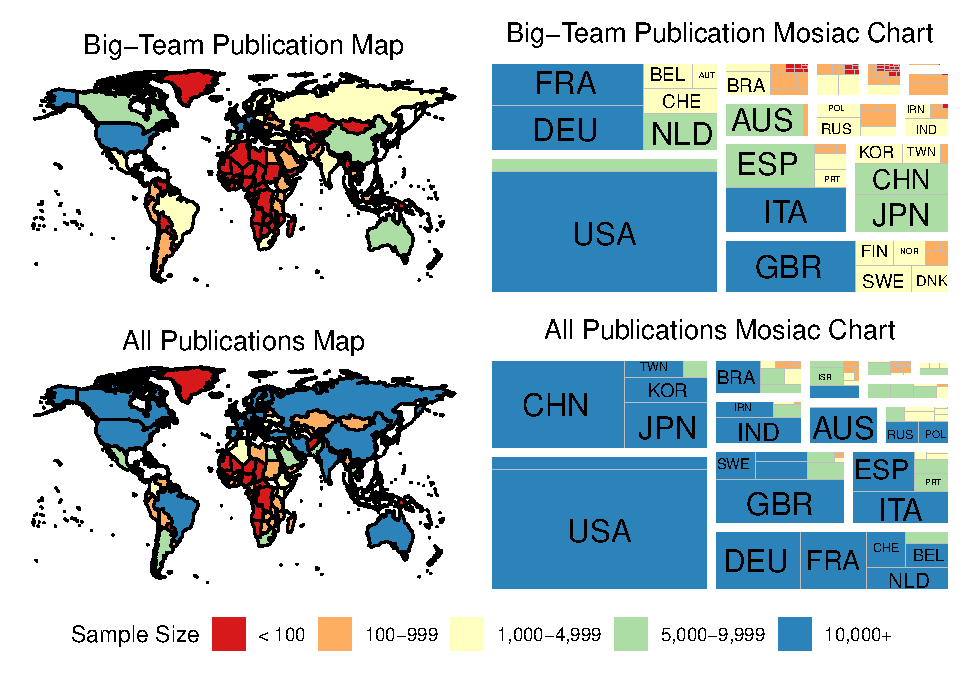
\includegraphics{manuscript_scopus_files/figure-latex/fig-map-both-1.pdf}
\caption{\label{fig:fig-map-both}Geopolitical regions represented in big-team science publications versus all publications.}
\end{figure}

Author geopoligical region is displayed in Figure \ref{fig:fig-map-both}. Big team publications appear to be lead by North America and Western Europe, while all publications are lead by North America and East Asia. To understand the change in representation diversity, we examined if the number of regions in a publication is predicted by the year of publication. Increasing diversity would be represented by a positive slope, while decreasing diversity would be represented by a negative slope. As shown in Figure \ref{fig:fig-heatmap}, the physical sciences do not show a trend of change in representation, while all other sciences showed a positive effect increasing in the number of geopolitical regions authors represent on publications.

Last, we examined the differences in representation for corresponding author sets versus all other authors. For papers with 10 to 49 authors, we used the three first authors and the last author to compare against other authors. For 50 to 99 authors, five first authors plus last were used, and for all papers with more than 100 authors, we used ten first authors and the last author as the corresponding author set. We then calculated the frequencies of each of the UN Sub-Regions for corresponding authors versus all other authors, converting these values to proportions. Given the expected small sample sizes of these contingency tables, we grouped together titles based on the year of publication. For each grouping, we then calculated the effect size of the differences in frequencies comparing corresponding authors to all other authors. Since this data is categorical, we used Cramer's \emph{V} to represent the effect size. If the effect size includes zero in its confidence interval (to four decimal places), this result will imply that first and all other authors represent the same pattern of UN Sub-Region diversity. Any confidence interval that does include zero represents a difference in diversity.

\begin{figure}
\centering
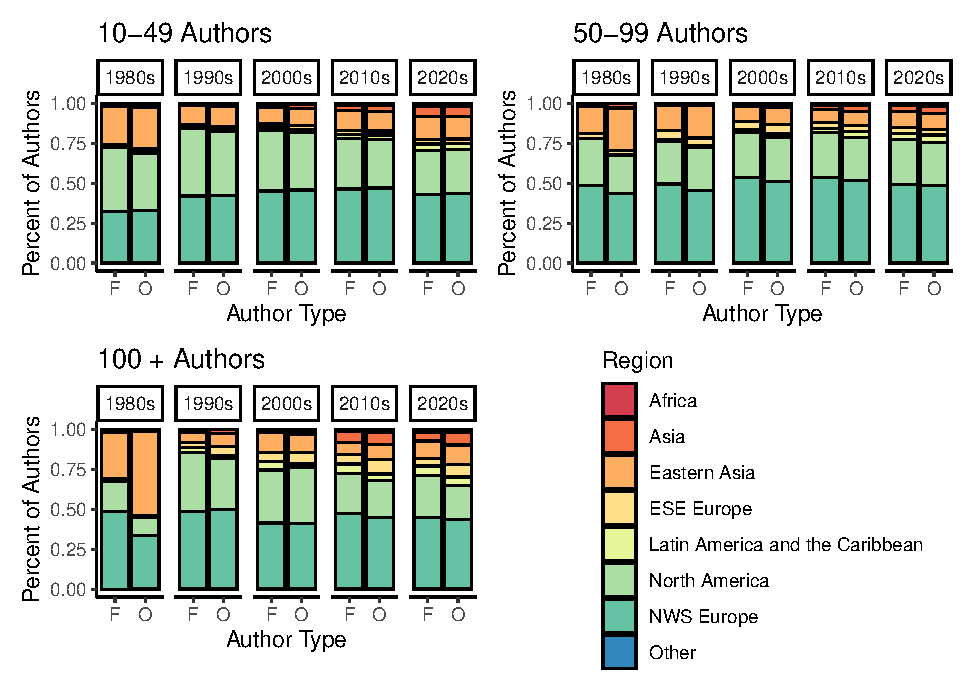
\includegraphics{manuscript_scopus_files/figure-latex/fig-author-gpe-1.pdf}
\caption{\label{fig:fig-author-gpe}A comparison of author affiliation geopolitical region across decades. F stands for first authors and O stands for other authors.}
\end{figure}

\begin{figure}
\centering
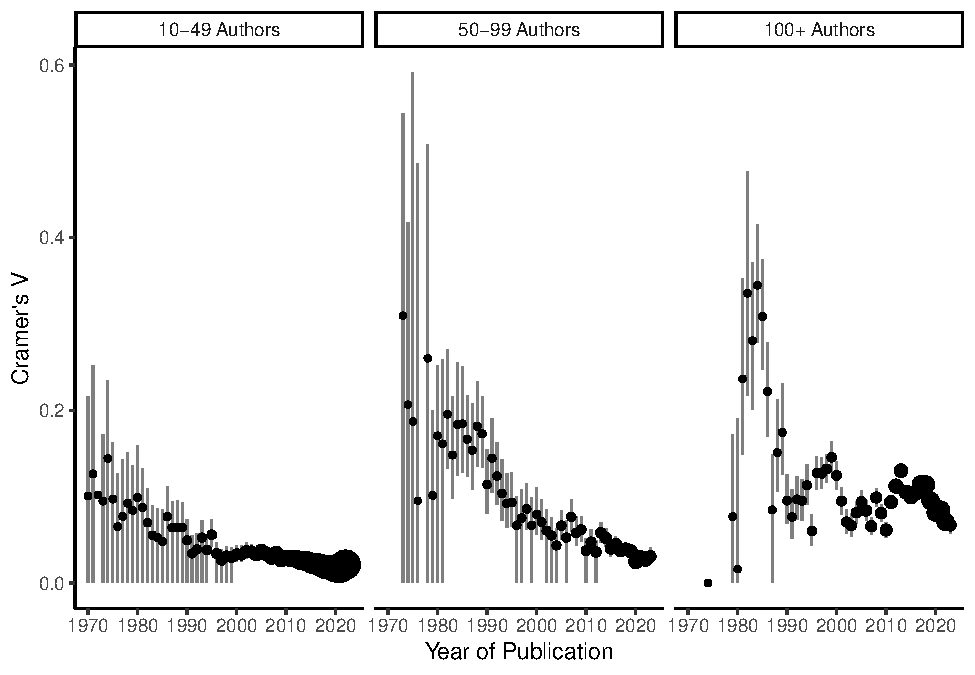
\includegraphics{manuscript_scopus_files/figure-latex/fig-effect-gpe-1.pdf}
\caption{\label{fig:fig-effect-gpe}Effect size of the differences in representation for UN Regions for author affiliations in big-team science papers by year. Larger dots indicate more papers and authors represented in the calculation of effect size.}
\end{figure}

Figure \ref{fig:fig-author-gpe} indicates the percent of authors in regions. In general, we found the same pattern as the overall analysis wherein most authors are from Europe and North America. The pattern of representation is roughly similar for the separation of small, medium, and large numbers of authors on papers. Across time, the representation does appear to diversify, with more representation in Asia, Latin American, and Africa. Figure \ref{fig:fig-effect-gpe} represents the size of the differences in first/corresponding authors and other authors across time and number of authors. The differences in representation are larger for papers with more authors; however, the effects are non-zero for many of the comparisons. Encouragingly, over time these effects appear to diminish in size. One limitation with the calculation of effect sizes for count data is the sensitivity of the data to sample size (i.e., \(\chi^2\) is upwardly biased by sample size, and \(V\) is calculated based on this value). While we used the inclusion of zero as our boundary for ``significance'', the interpretation of the effects is that most are likely small: \(V\) \textless{} .05: 31.79\%, \textless{} .10: 70.20\%, \textless{} .20: 94.04\%.

\hypertarget{discussion}{%
\section{Discussion}\label{discussion}}

\begin{itemize}
\tightlist
\item
  number of publications increasing
\item
  research areas appear to be cancer, physics, and psychology
\item
  the number of authors is increasing as well
\item
  career length is decreasing, number of publications necessary to be involved is decreasing
\item
  number of gpe increasing
\item
  appears to be slowly diversifying, yet still not equal in first and other authors in diversity
\end{itemize}

limitations - based on the data we could get, we made up the definition of BTS, under-representation of articles in other languages/that they don't collect

future: incentives for bts and why people do it

\newpage

\hypertarget{references}{%
\section{References}\label{references}}

\begingroup
\setlength{\parindent}{-0.5in}
\setlength{\leftskip}{0.5in}

\hypertarget{refs}{}
\begin{CSLReferences}{1}{0}
\leavevmode\vadjust pre{\hypertarget{ref-aphilos2021}{}}%
A philosophical case for big physics. (2021). \emph{Nature Physics}, \emph{17}(6), 661--661. \url{https://doi.org/10.1038/s41567-021-01278-0}

\leavevmode\vadjust pre{\hypertarget{ref-allen2019}{}}%
Allen, L., O'Connell, A., \& Kiermer, V. (2019). How can we ensure visibility and diversity in research contributions? How the Contributor Role Taxonomy (CRediT) is helping the shift from authorship to contributorship. \emph{Learned Publishing}, \emph{32}(1), 71--74. \url{https://doi.org/10.1002/leap.1210}

\leavevmode\vadjust pre{\hypertarget{ref-auspurg2021has}{}}%
Auspurg, K., \& Brüderl, J. (2021). Has the credibility of the social sciences been credibly destroyed? Reanalyzing the {``}many analysts, one data set{''} project. \emph{Socius : Sociological Research for a Dynamic World}, \emph{7}, 23780231211024420.

\leavevmode\vadjust pre{\hypertarget{ref-bago2022}{}}%
Bago, B., Kovacs, M., Protzko, J., Nagy, T., Kekecs, Z., Palfi, B., \ldots{} Aczel, B. (2022). Situational factors shape moral judgements in the trolley dilemma in Eastern, Southern and Western countries in a culturally diverse sample. \emph{Nature Human Behaviour}, 1--13. \url{https://doi.org/10.1038/s41562-022-01319-5}

\leavevmode\vadjust pre{\hypertarget{ref-buttrick2020}{}}%
Buttrick, N. R., Aczel, B., Aeschbach, L. F., Bakos, B. E., Brühlmann, F., Claypool, H. M., \ldots{} Wood, M. J. (2020). Many Labs 5: Registered Replication of Vohs and Schooler (2008), Experiment 1. \emph{Advances in Methods and Practices in Psychological Science}, \emph{3}(3), 429--438. \url{https://doi.org/10.1177/2515245920917931}

\leavevmode\vadjust pre{\hypertarget{ref-castelnovo2018}{}}%
Castelnovo, P., Florio, M., Forte, S., Rossi, L., \& Sirtori, E. (2018). The economic impact of technological procurement for large-scale research infrastructures: Evidence from the Large Hadron Collider at CERN. \emph{Research Policy}, \emph{47}(9), 1853--1867. \url{https://doi.org/10.1016/j.respol.2018.06.018}

\leavevmode\vadjust pre{\hypertarget{ref-coles2022}{}}%
Coles, N. A., Hamlin, J. K., Sullivan, L. L., Parker, T. H., \& Altschul, D. (2022). Build up big-team science. \emph{Nature}, \emph{601}(7894), 505--507. \url{https://doi.org/10.1038/d41586-022-00150-2}

\leavevmode\vadjust pre{\hypertarget{ref-collins2003}{}}%
Collins, F. S., Morgan, M., \& Patrinos, A. (2003). The human genome project: Lessons from large-scale biology. \emph{Science}, \emph{300}(5617), 286--290. \url{https://doi.org/10.1126/science.1084564}

\leavevmode\vadjust pre{\hypertarget{ref-dorison2022}{}}%
Dorison, C., Lerner, J., Heller, B., Rothman, A., Kawachi, I., Wang, K., \ldots{} Coles, N. (2022). A global test of message framing on behavioural intentions, policy support, information seeking, and experienced anxiety during the COVID-19 pandemic. \emph{Affective Science}. \url{https://doi.org/10.31234/osf.io/sevkf}

\leavevmode\vadjust pre{\hypertarget{ref-ebersole2016}{}}%
Ebersole, C. R., Atherton, O. E., Belanger, A. L., Skulborstad, H. M., Allen, J. M., Banks, J. B., \ldots{} Nosek, B. A. (2016). Many Labs 3: Evaluating participant pool quality across the academic semester via replication. \emph{Journal of Experimental Social Psychology}, \emph{67}, 68--82. \url{https://doi.org/10.1016/j.jesp.2015.10.012}

\leavevmode\vadjust pre{\hypertarget{ref-ebersole2020}{}}%
Ebersole, C. R., Mathur, M. B., Baranski, E., Bart-Plange, D.-J., Buttrick, N. R., Chartier, C. R., \ldots{} Nosek, B. A. (2020). Many Labs 5: Testing Pre-Data-Collection Peer Review as an Intervention to Increase Replicability. \emph{Advances in Methods and Practices in Psychological Science}, \emph{3}(3), 309--331. \url{https://doi.org/10.1177/2515245920958687}

\leavevmode\vadjust pre{\hypertarget{ref-10.7554ux2feLife.71601}{}}%
Errington, T. M., Mathur, M., Soderberg, C. K., Denis, A., Perfito, N., Iorns, E., \& Nosek, B. A. (2021). Investigating the replicability of preclinical cancer biology. \emph{eLife}, \emph{10}, e71601. \url{https://doi.org/10.7554/eLife.71601}

\leavevmode\vadjust pre{\hypertarget{ref-forscher2020}{}}%
Forscher, P. S., Wagenmakers, E.-J., Coles, N. A., Silan, M. A. A., Dutra, N. B., Basnight-Brown, D., \& IJzerman, H. (2020). \emph{The benefits, barriers, and risks of big team science}. \url{https://doi.org/10.31234/osf.io/2mdxh}

\leavevmode\vadjust pre{\hypertarget{ref-franco2014}{}}%
Franco, A., Malhotra, N., \& Simonovits, G. (2014). Publication bias in the social sciences: Unlocking the file drawer. \emph{Science}, \emph{345}(6203), 1502--1505. \url{https://doi.org/10.1126/science.1255484}

\leavevmode\vadjust pre{\hypertarget{ref-grahe2014}{}}%
Grahe, J. E. (2014). Announcing open science badges and reaching for the sky. \emph{The Journal of Social Psychology}, \emph{154}(1), 1--3. \url{https://doi.org/10.1080/00224545.2014.853582}

\leavevmode\vadjust pre{\hypertarget{ref-henrich2010}{}}%
Henrich, J., Heine, S. J., \& Norenzayan, A. (2010). The weirdest people in the world? \emph{Behavioral and Brain Sciences}, \emph{33}(2-3), 61--83. \url{https://doi.org/10.1017/S0140525X0999152X}

\leavevmode\vadjust pre{\hypertarget{ref-hubbard1997}{}}%
Hubbard, R., \& Armstrong, J. S. (1997). Publication Bias against Null Results. \emph{Psychological Reports}, \emph{80}(1), 337--338. \url{https://doi.org/10.2466/pr0.1997.80.1.337}

\leavevmode\vadjust pre{\hypertarget{ref-ioannidis2015}{}}%
Ioannidis, J. P. A. (2015). Failure to replicate: Sound the alarm. \emph{Cerebrum: The Dana Forum on Brain Science}, \emph{2015}. Retrieved from \url{https://www.ncbi.nlm.nih.gov/pmc/articles/PMC4938249/}

\leavevmode\vadjust pre{\hypertarget{ref-isager2021}{}}%
Isager, P. M., Aert, R. C. M. van, Bahník, Š., Brandt, M. J., DeSoto, K. A., Giner-Sorolla, R., \ldots{} Lakens, D. (2021a). Deciding what to replicate: A decision model for replication study selection under resource and knowledge constraints. \emph{Psychological Methods}. \url{https://doi.org/10.1037/met0000438}

\leavevmode\vadjust pre{\hypertarget{ref-isager2021a}{}}%
Isager, P. M., Aert, R. C. M. van, Bahník, Š., Brandt, M. J., DeSoto, K. A., Giner-Sorolla, R., \ldots{} Lakens, D. (2021b). Deciding what to replicate: A decision model for replication study selection under resource and knowledge constraints. \emph{Psychological Methods}. \url{https://doi.org/10.1037/met0000438}

\leavevmode\vadjust pre{\hypertarget{ref-john2012}{}}%
John, L. K., Loewenstein, G., \& Prelec, D. (2012). Measuring the Prevalence of Questionable Research Practices With Incentives for Truth Telling. \emph{Psychological Science}, \emph{23}(5), 524--532. \url{https://doi.org/10.1177/0956797611430953}

\leavevmode\vadjust pre{\hypertarget{ref-jones2021}{}}%
Jones, B. C., DeBruine, L. M., Flake, J. K., Liuzza, M. T., Antfolk, J., Arinze, N. C., \ldots{} Coles, N. A. (2021). To which world regions does the valence{\textendash}dominance model of social perception apply? \emph{Nature Human Behaviour}, \emph{5}(1), 159--169. \url{https://doi.org/10.1038/s41562-020-01007-2}

\leavevmode\vadjust pre{\hypertarget{ref-kidwell2016}{}}%
Kidwell, M. C., Lazarević, L. B., Baranski, E., Hardwicke, T. E., Piechowski, S., Falkenberg, L.-S., \ldots{} Nosek, B. A. (2016). Badges to Acknowledge Open Practices: A Simple, Low-Cost, Effective Method for Increasing Transparency. \emph{PLOS Biology}, \emph{14}(5), e1002456. \url{https://doi.org/10.1371/journal.pbio.1002456}

\leavevmode\vadjust pre{\hypertarget{ref-klein2022}{}}%
Klein, Richard A., Cook, C. L., Ebersole, C. R., Vitiello, C., Nosek, B. A., Hilgard, J., \ldots{} Ratliff, K. A. (2022). Many Labs 4: Failure to Replicate Mortality Salience Effect With and Without Original Author Involvement. \emph{Collabra: Psychology}, \emph{8}(1), 35271. \url{https://doi.org/10.1525/collabra.35271}

\leavevmode\vadjust pre{\hypertarget{ref-klein2018}{}}%
Klein, Richard A., Vianello, M., Hasselman, F., Adams, B. G., Adams, R. B., Alper, S., \ldots{} Nosek, B. A. (2018). Many Labs 2: Investigating Variation in Replicability Across Samples and Settings. \emph{Advances in Methods and Practices in Psychological Science}, \emph{1}(4), 443--490. \url{https://doi.org/10.1177/2515245918810225}

\leavevmode\vadjust pre{\hypertarget{ref-lebel2018}{}}%
LeBel, E. P., McCarthy, R. J., Earp, B. D., Elson, M., \& Vanpaemel, W. (2018). A Unified Framework to Quantify the Credibility of Scientific Findings. \emph{Advances in Methods and Practices in Psychological Science}, \emph{1}(3), 389--402. \url{https://doi.org/10.1177/2515245918787489}

\leavevmode\vadjust pre{\hypertarget{ref-legate2022}{}}%
Legate, N., Nguyen, T., Weinstein, N., Moller, A., Legault, L., Maniaci, M. R., \ldots{} Primbs, M. (2022). A global experiment on motivating social distancing during the COVID-19 pandemic. \emph{Proceedings of the National Academy of Sciences}. \url{https://doi.org/10.31234/osf.io/n3dyf}

\leavevmode\vadjust pre{\hypertarget{ref-maizey2019}{}}%
Maizey, L., \& Tzavella, L. (2019). Barriers and solutions for early career researchers in tackling the reproducibility crisis in cognitive neuroscience. \emph{Cortex}, \emph{113}, 357--359. \url{https://doi.org/10.1016/j.cortex.2018.12.015}

\leavevmode\vadjust pre{\hypertarget{ref-mathur2020}{}}%
Mathur, M. B., Bart-Plange, D.-J., Aczel, B., Bernstein, M. H., Ciunci, A. M., Ebersole, C. R., \ldots{} Frank, M. C. (2020). Many Labs 5: Registered Multisite Replication of the Tempting-Fate Effects in Risen and Gilovich (2008). \emph{Advances in Methods and Practices in Psychological Science}, \emph{3}(3), 394--404. \url{https://doi.org/10.1177/2515245918785165}

\leavevmode\vadjust pre{\hypertarget{ref-maxwell2015}{}}%
Maxwell, S. E., Lau, M. Y., \& Howard, G. S. (2015). Is psychology suffering from a replication crisis?: What does 'failure to replicate' really mean? \emph{American Psychologist}, \emph{70}(6), 487--498. \url{https://doi.org/10.1037/a0039400}

\leavevmode\vadjust pre{\hypertarget{ref-mayo-wilson2021}{}}%
Mayo-Wilson, E., Grant, S., Supplee, L., Kianersi, S., Amin, A., DeHaven, A., \& Mellor, D. (2021). Evaluating implementation of the transparency and openness promotion~(TOP) guidelines:~The TRUST process for rating journal policies, procedures, and practices. \emph{Research Integrity and Peer Review}, \emph{6}(1), 9. \url{https://doi.org/10.1186/s41073-021-00112-8}

\leavevmode\vadjust pre{\hypertarget{ref-moshontz2018}{}}%
Moshontz, H., Campbell, L., Ebersole, C. R., IJzerman, H., Urry, H. L., Forscher, P. S., \ldots{} Chartier, C. R. (2018). The Psychological Science Accelerator: Advancing Psychology Through a Distributed Collaborative Network. \emph{Advances in Methods and Practices in Psychological Science}, \emph{1}(4), 501--515. \url{https://doi.org/10.1177/2515245918797607}

\leavevmode\vadjust pre{\hypertarget{ref-nelson2018}{}}%
Nelson, L. D., Simmons, J., \& Simonsohn, U. (2018). Psychology's renaissance. \emph{Annual Review of Psychology}, \emph{69}(1), 511--534. \url{https://doi.org/10.1146/annurev-psych-122216-011836}

\leavevmode\vadjust pre{\hypertarget{ref-newson2021}{}}%
Newson, M., Buhrmester, M., Xygalatas, D., \& Whitehouse, H. (2021). Go WILD, not WEIRD. \emph{Journal for the Cognitive Science of Religion}, \emph{6}(1-2). \url{https://doi.org/10.1558/jcsr.38413}

\leavevmode\vadjust pre{\hypertarget{ref-nosek2015}{}}%
Nosek, B. A., Alter, G., Banks, G. C., Borsboom, D., Bowman, S. D., Breckler, S. J., \ldots{} Yarkoni, T. (2015). Promoting an open research culture. \emph{Science}, \emph{348}(6242), 1422--1425. \url{https://doi.org/10.1126/science.aab2374}

\leavevmode\vadjust pre{\hypertarget{ref-nosek2014method}{}}%
Nosek, Brian A., \& Lakens, D. (2014a). A method to increase the credibility of published results. \emph{Social Psychology}, \emph{45}(3), 137141.

\leavevmode\vadjust pre{\hypertarget{ref-nosek2014}{}}%
Nosek, Brian A., \& Lakens, D. (2014b). Registered Reports: A Method to Increase the Credibility of Published Results. \emph{Social Psychology}, \emph{45}(3), 137--141. \url{https://doi.org/10.1027/1864-9335/a000192}

\leavevmode\vadjust pre{\hypertarget{ref-nosek2012}{}}%
Nosek, Brian A., Spies, J. R., \& Motyl, M. (2012). Scientific Utopia: II. Restructuring Incentives and Practices to Promote Truth Over Publishability. \emph{Perspectives on Psychological Science}, \emph{7}(6), 615--631. \url{https://doi.org/10.1177/1745691612459058}

\leavevmode\vadjust pre{\hypertarget{ref-oed2016}{}}%
OED. (2016). \emph{Collaboration}. Oxford: Oxford University.

\leavevmode\vadjust pre{\hypertarget{ref-opensciencecollaboration2015}{}}%
Open Science Collaboration. (2015). Estimating the reproducibility of psychological science. \emph{Science}, \emph{349}(6251), aac4716--aac4716. \url{https://doi.org/10.1126/science.aac4716}

\leavevmode\vadjust pre{\hypertarget{ref-rad2018}{}}%
Rad, M. S., Martingano, A. J., \& Ginges, J. (2018). Toward a psychology of homo sapiens: Making psychological science more representative of the human population. \emph{Proceedings of the National Academy of Sciences}, \emph{115}(45), 11401--11405. \url{https://doi.org/10.1073/pnas.1721165115}

\leavevmode\vadjust pre{\hypertarget{ref-silberzahn2018many}{}}%
Silberzahn, R., Uhlmann, E. L., Martin, D. P., Anselmi, P., Aust, F., Awtrey, E., \ldots{} others. (2018). Many analysts, one data set: Making transparent how variations in analytic choices affect results. \emph{Advances in Methods and Practices in Psychological Science}, \emph{1}(3), 337356.

\leavevmode\vadjust pre{\hypertarget{ref-skorb2020}{}}%
Skorb, L., Aczel, B., Bakos, B. E., Feinberg, L., Hałasa, E., Kauff, M., \ldots{} Hartshorne, J. K. (2020). Many Labs 5: Replication of van Dijk, van Kleef, Steinel, and van Beest (2008). \emph{Advances in Methods and Practices in Psychological Science}, \emph{3}(3), 418--428. \url{https://doi.org/10.1177/2515245920927643}

\leavevmode\vadjust pre{\hypertarget{ref-stewart2017}{}}%
Stewart, N., Chandler, J., \& Paolacci, G. (2017). Crowdsourcing samples in cognitive science. \emph{Trends in Cognitive Sciences}, \emph{21}(10), 736--748. \url{https://doi.org/10.1016/j.tics.2017.06.007}

\leavevmode\vadjust pre{\hypertarget{ref-stewart2020}{}}%
Stewart, S., Rinke, E. M., McGarrigle, R., Lynott, D., Lunny, C., Lautarescu, A., \ldots{} Crook, Z. (2020). \emph{Pre-registration and registered reports: A primer from UKRN}. \url{https://doi.org/10.31219/osf.io/8v2n7}

\leavevmode\vadjust pre{\hypertarget{ref-vanbavel2022}{}}%
Van Bavel, J. J., Cichocka, A., Capraro, V., Sjåstad, H., Nezlek, J. B., Pavlović, T., \ldots{} Boggio, P. S. (2022). National identity predicts public health support during a global pandemic. \emph{Nature Communications}, \emph{13}(1), 517. \url{https://doi.org/10.1038/s41467-021-27668-9}

\leavevmode\vadjust pre{\hypertarget{ref-vazire2022}{}}%
Vazire, S., Schiavone, S. R., \& Bottesini, J. G. (2022). Credibility Beyond Replicability: Improving the Four Validities in Psychological Science. \emph{Current Directions in Psychological Science}, \emph{31}(2), 162--168. \url{https://doi.org/10.1177/09637214211067779}

\leavevmode\vadjust pre{\hypertarget{ref-wang2021}{}}%
Wang, K., Goldenberg, A., Dorison, C. A., Miller, J. K., Uusberg, A., Lerner, J. S., \ldots{} Moshontz, H. (2021). A multi-country test of brief reappraisal interventions on emotions during the COVID-19 pandemic. \emph{Nature Human Behaviour}, \emph{5}(8), 1089--1110. \url{https://doi.org/10.1038/s41562-021-01173-x}

\leavevmode\vadjust pre{\hypertarget{ref-zwaan2018}{}}%
Zwaan, R. A., Etz, A., Lucas, R. E., \& Donnellan, M. B. (2018). Making replication mainstream. \emph{Behavioral and Brain Sciences}, \emph{41}, e120. \url{https://doi.org/10.1017/S0140525X17001972}

\end{CSLReferences}

\endgroup

\newpage

\hypertarget{appendix-appendix}{%
\appendix}


\hypertarget{supplemental-materials}{%
\section{Supplemental Materials}\label{supplemental-materials}}

\hypertarget{rq1-publisher-information.-2}{%
\subsection{RQ1: Publisher Information.}\label{rq1-publisher-information.-2}}

\textbf{Number of Journals}.

Table \ref{tab:tab-snip} indicates the SNIP values for BTS publications, while Table \ref{tab:tab-snip-all}. The results from these tables indicate that impact values are slightly higher for BTS publications, while the overall median, minimum, and maximum are the same for each grouping.

\begin{table}[tbp]

\begin{center}
\begin{threeparttable}

\caption{\label{tab:tab-snip}Big-Team Science SNIP Values}

\begin{tabular}{llllll}
\toprule
Subject Area & \multicolumn{1}{c}{M} & \multicolumn{1}{c}{SD} & \multicolumn{1}{c}{Minimum} & \multicolumn{1}{c}{Median} & \multicolumn{1}{c}{Maximum}\\
\midrule
Health Sciences & 2.36 & 3.59 & 0.00 & 1.58 & 173.93\\
Physical Sciences & 1.57 & 1.17 & 0.00 & 1.27 & 30.40\\
Social Sciences & 1.94 & 1.72 & 0.00 & 1.52 & 30.40\\
Life Sciences & 2.02 & 1.60 & 0.00 & 1.51 & 19.07\\
\bottomrule
\end{tabular}

\end{threeparttable}
\end{center}

\end{table}

\begin{table}[tbp]

\begin{center}
\begin{threeparttable}

\caption{\label{tab:tab-snip-all}All Journal Articles SNIP Values}

\begin{tabular}{llllll}
\toprule
Subject Area & \multicolumn{1}{c}{M} & \multicolumn{1}{c}{SD} & \multicolumn{1}{c}{Minimum} & \multicolumn{1}{c}{Median} & \multicolumn{1}{c}{Maximum}\\
\midrule
Health Sciences & 1.45 & 2.87 & 0.00 & 1.15 & 173.93\\
Physical Sciences & 1.08 & 0.77 & 0.00 & 0.97 & 30.40\\
Social Sciences & 1.32 & 1.03 & 0.00 & 1.15 & 30.40\\
Life Sciences & 1.19 & 0.86 & 0.00 & 1.06 & 19.07\\
\bottomrule
\end{tabular}

\end{threeparttable}
\end{center}

\end{table}

\hypertarget{rq2-publication-information.-2}{%
\subsection{RQ2: Publication Information.}\label{rq2-publication-information.-2}}

\textbf{Keywords}. Figure \ref{fig:fig-keywords} indicates the most common keywords present for the BTS publications by subject area. The keywords were tokenized into single tokens. Keywords were then lowercased, and all stop words (for example, the, an, of, into, for) were removed. Finally, a frequency count of tokens was tabulated for each subject area, and this count is used to create the final word cloud presented.

\begin{figure}
\centering
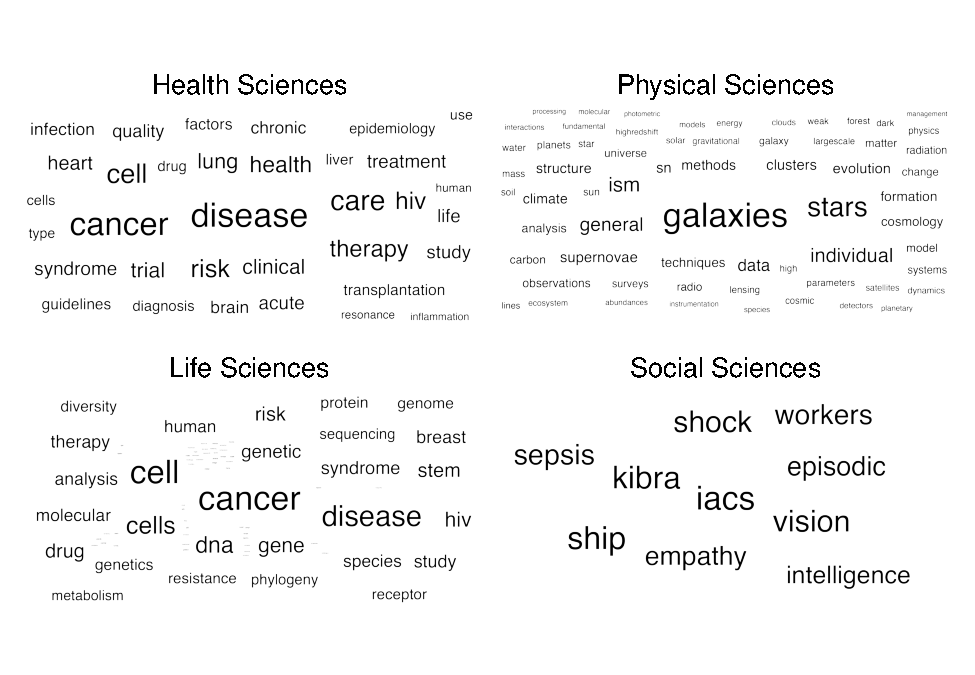
\includegraphics{manuscript_scopus_files/figure-latex/fig-keywords-1.pdf}
\caption{\label{fig:fig-keywords}Keyword Analysis for Each of the Four Subject Areas.}
\end{figure}

\hypertarget{rq3-authors}{%
\subsection{RQ3: Authors}\label{rq3-authors}}

\textbf{Institution}.

Institution was normalized by taking the total number of unique institutions and dividing by the total number of institution listings. The patterns are similar for each decade in that papers are often either half unique institutions or mostly unique institutions overall as show in Figure \ref{fig:fig-inst}.

\begin{figure}
\centering
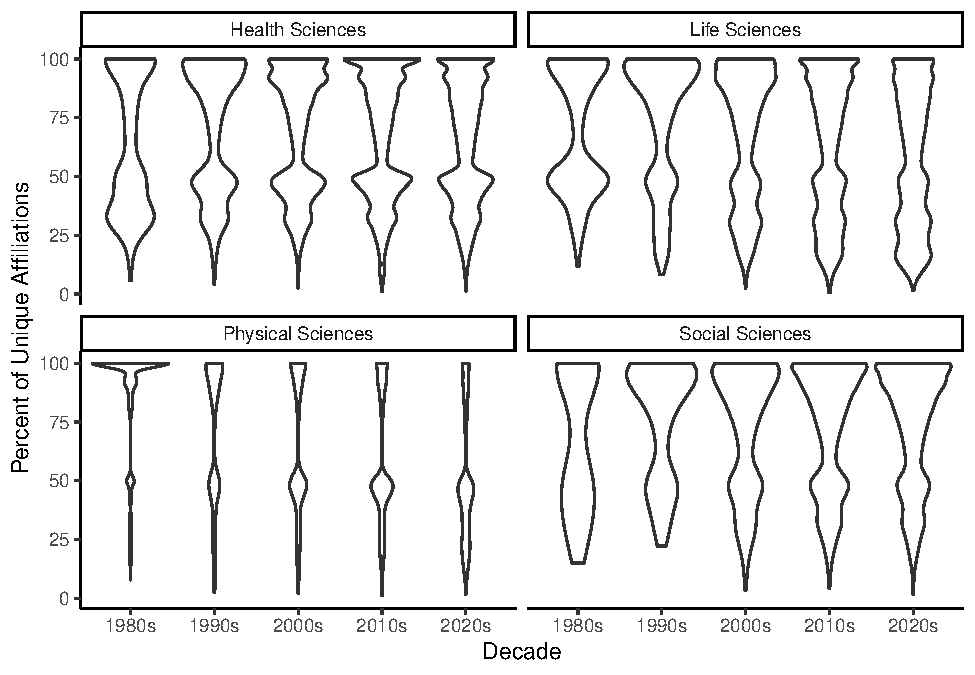
\includegraphics{manuscript_scopus_files/figure-latex/fig-inst-1.pdf}
\caption{\label{fig:fig-inst}Number of unique institutions involved in big-team science papers across decades.}
\end{figure}

\textbf{\emph{Education}}. As noted in our pre-registration, we would only present this variable if we could obtain at least 50\% information on the authors who publish in big team science papers. 95.83\% of the data was not available.

\textbf{\emph{Types of Publications}}.

Types of publications are presented in Figure \ref{fig:fig-pub-types}. The patterns of publications are roughly similar for big team science authors and all authors. It appears that porportionally, big team members are more likely to post preprints in comparison to all authors.

\begin{figure}
\centering
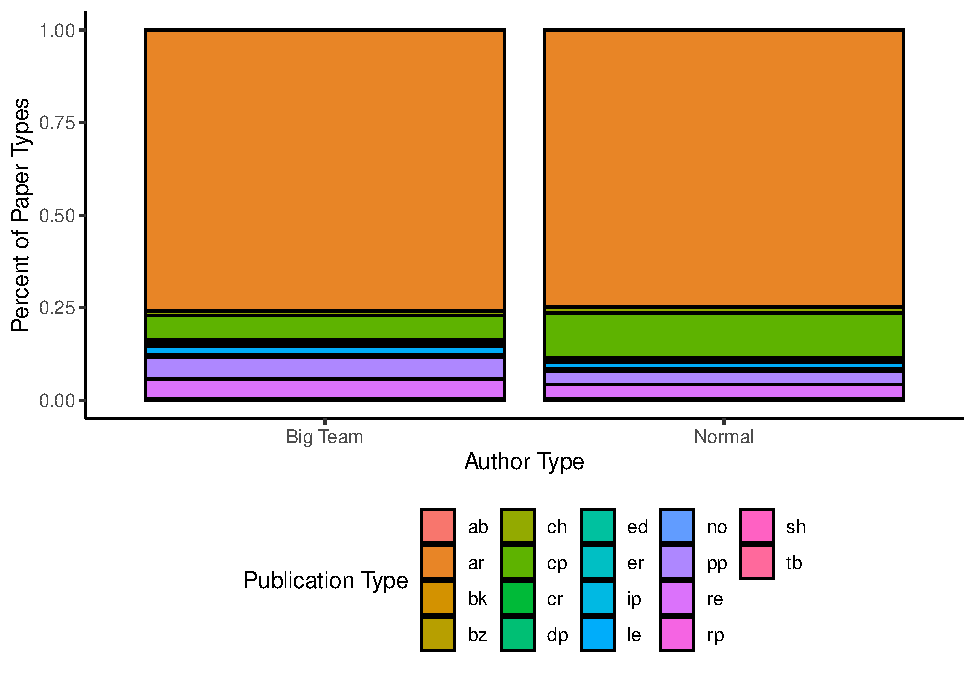
\includegraphics{manuscript_scopus_files/figure-latex/fig-pub-types-1.pdf}
\caption{\label{fig:fig-pub-types}Types of publications for big-team science and all authors.}
\end{figure}


\end{document}
